% This is LLNCS.DEM the demonstration file of
% the LaTeX macro package from Springer-Verlag
% for Lecture Notes in Computer Science,
% version 2.4 for LaTeX2e as of 16. April 2010
%
\documentclass{llncs}
%
\usepackage{makeidx}  % allows for indexgeneration
\usepackage{graphicx}
\usepackage{subcaption}
\usepackage[utf8]{inputenc}


%
\begin{document}
%
\frontmatter          % for the preliminaries
%
\pagestyle{headings}  % switches on printing of running heads
\addtocmark{Hamiltonian Mechanics} % additional mark in the TOC
%
%
\mainmatter              % start of the contributions
%
\title{Latenzvergleich bei PC zu Smartphone Audioübertragungsanwendungen}
%
\titlerunning{Hamiltonian Mechanics}  % abbreviated title (for running head)
%                                     also used for the TOC unless
%                                     \toctitle is used
%
\author{Florian Kovacs, Johannes Hasreiter \and Christian Reiser}
%
\authorrunning{Ivar Ekeland et al.} % abbreviated author list (for running head)
%
%%%% list of authors for the TOC (use if author list has to be modified)
\tocauthor{Ivar Ekeland, Roger Temam, Jeffrey Dean, David Grove,
Craig Chambers, Kim B. Bruce, and Elisa Bertino}
%
\institute{Universit\"at Passau}

\maketitle              % typeset the title of the contribution

\begin{abstract}
TODO
\end{abstract}
%
\section{Android-Anwendung als Ersatz für drahtlose Kopfhörer}
Drahtlose Kopfhörer haben in den letzten Jahren an Beliebtheit gewonnen. Viele NutzerInnen besitzen jedoch bereits hochqualitative kabelgebundene Kopfhörer, wollen von den Vorteilen der Drahtlosigkeit profitieren, aber gleichzeitig nicht in neue Kopfhörer investieren. Abhilfe können Android-Anwendungen verschaffen, die die Tonausgabe des PCs der NutzerIn über WiFi an ihr Smartphone weiterleiten. An das Smartphone werden lediglich herkömmliche Kopfhörer angeschlossen. Die NutzerIn gewinnt damit Bewegungsfreiheit in einem ähnlichen Maße, wie es bei der Verwendung von drahtlosen Kopfhörern der Fall ist. Für das Ansehen von Videos, ist es erforderlich, dass Ton- und Bildausgabe möglichst synchron sind. Insbesondere bei Videos mit sprechenden Menschen kann es als störend empfunden werden, wenn der Ton verzögert abgespielt wird. Möchte die NutzerIn eine Übertragungsanwendung zum Ansehen von Filmen verwenden, ist es deshalb von zentraler Bedeutung, dass der Ton mit möglichst geringer Latenz abgespielt wird. Aus diesem Grund vergleichen wir in dieser Studie die Audiolatenz mehrerer Android-Anwendungen mit dem Ziel, diejenige mit der geringsten Latenz zu bestimmen und so der NutzerIn die Wahl einer geeigneten App zu erleichtern.

\section{Vorgehensweise}
In dieser Studie werden nur Anwendungen für das mobile Betriebssystem Android betrachtet. Da der Marktanteil von Android fast 90\% beträgt, ist dennoch ein Großteil der potenziellen NutzerInnen abgedeckt. Evaluiert werden die Anwendungen SoundWire (SW), TeamSpeak (TS) und WiFi Speaker (WFS).  Laut bestem Wissen der Autoren sind SW und WFS die einzigen beiden im Play Store verfügbaren Anwendungen, die die gewünschte Funktionalität bereitstellen (Stand: Januar 2017). Bei TS handelt es sich um eine VoIP-Anwendung, die aber so konfiguriert werden kann, dass sie ebenfalls über WiFi die Tonausgabe des PCs überträgt.

Eine herkömmliche Art die Latenz zu bestimmen, geht über das zusätzliche Senden des Zeitpunkts an dem die Tonwiedergabe am PC erfolgt ist. Die Differenz zwischen dem Zeitpunkt an dem die Tonwiedergabe am Smartphone stattgefunden hat und dem mitgesendeten Zeitpunkt entspricht der Latenz. Um diese Art der Messung durchzuführen, ist jedoch der Zugriff auf den Quellcode oder einer entsprechenden Schnittstelle der untersuchten Anwendung erforderlich. Da alle untersuchten Anwendungen proprietär sind, besteht nicht die Möglichkeit die Latenzmessungen derart durchzuführen.

Um dieses Problem zu umgehen, verwenden wir eine andere Art der Messung. Hierzu wird auf dem PC wiederholt ein Testton abgespielt. Aufgrund der Übertragungsanwendung wird der Ton verzögert auch auf dem Smartphone abgespielt. Währenddessen verwenden wir ein Mikrofon zur Aufzeichnung der Audioausgaben beider Geräte. In der anschließenden Analyse der Aufzeichnung, kann man anhand des Spektrogramms die Latenz bestimmen, vgl. Abb. 1. Vorteilhaft an diesem Ansatz ist, dass hier die Ende-zu-Ende-Verzögerung einschließlich aller Puffer-, Enkodier-, Dekodier- und Netzwerklatenzen gemessen wird. Werden programmatisch bestimmte Timestamps verwendet, besteht die Gefahr, dass die Erfassungsstelle der Timestamps falsch gewählt ist und somit bestimmte Latenzzeiten nicht ins Ergebnis einfließen.

\begin{figure}
	\begin{center}
		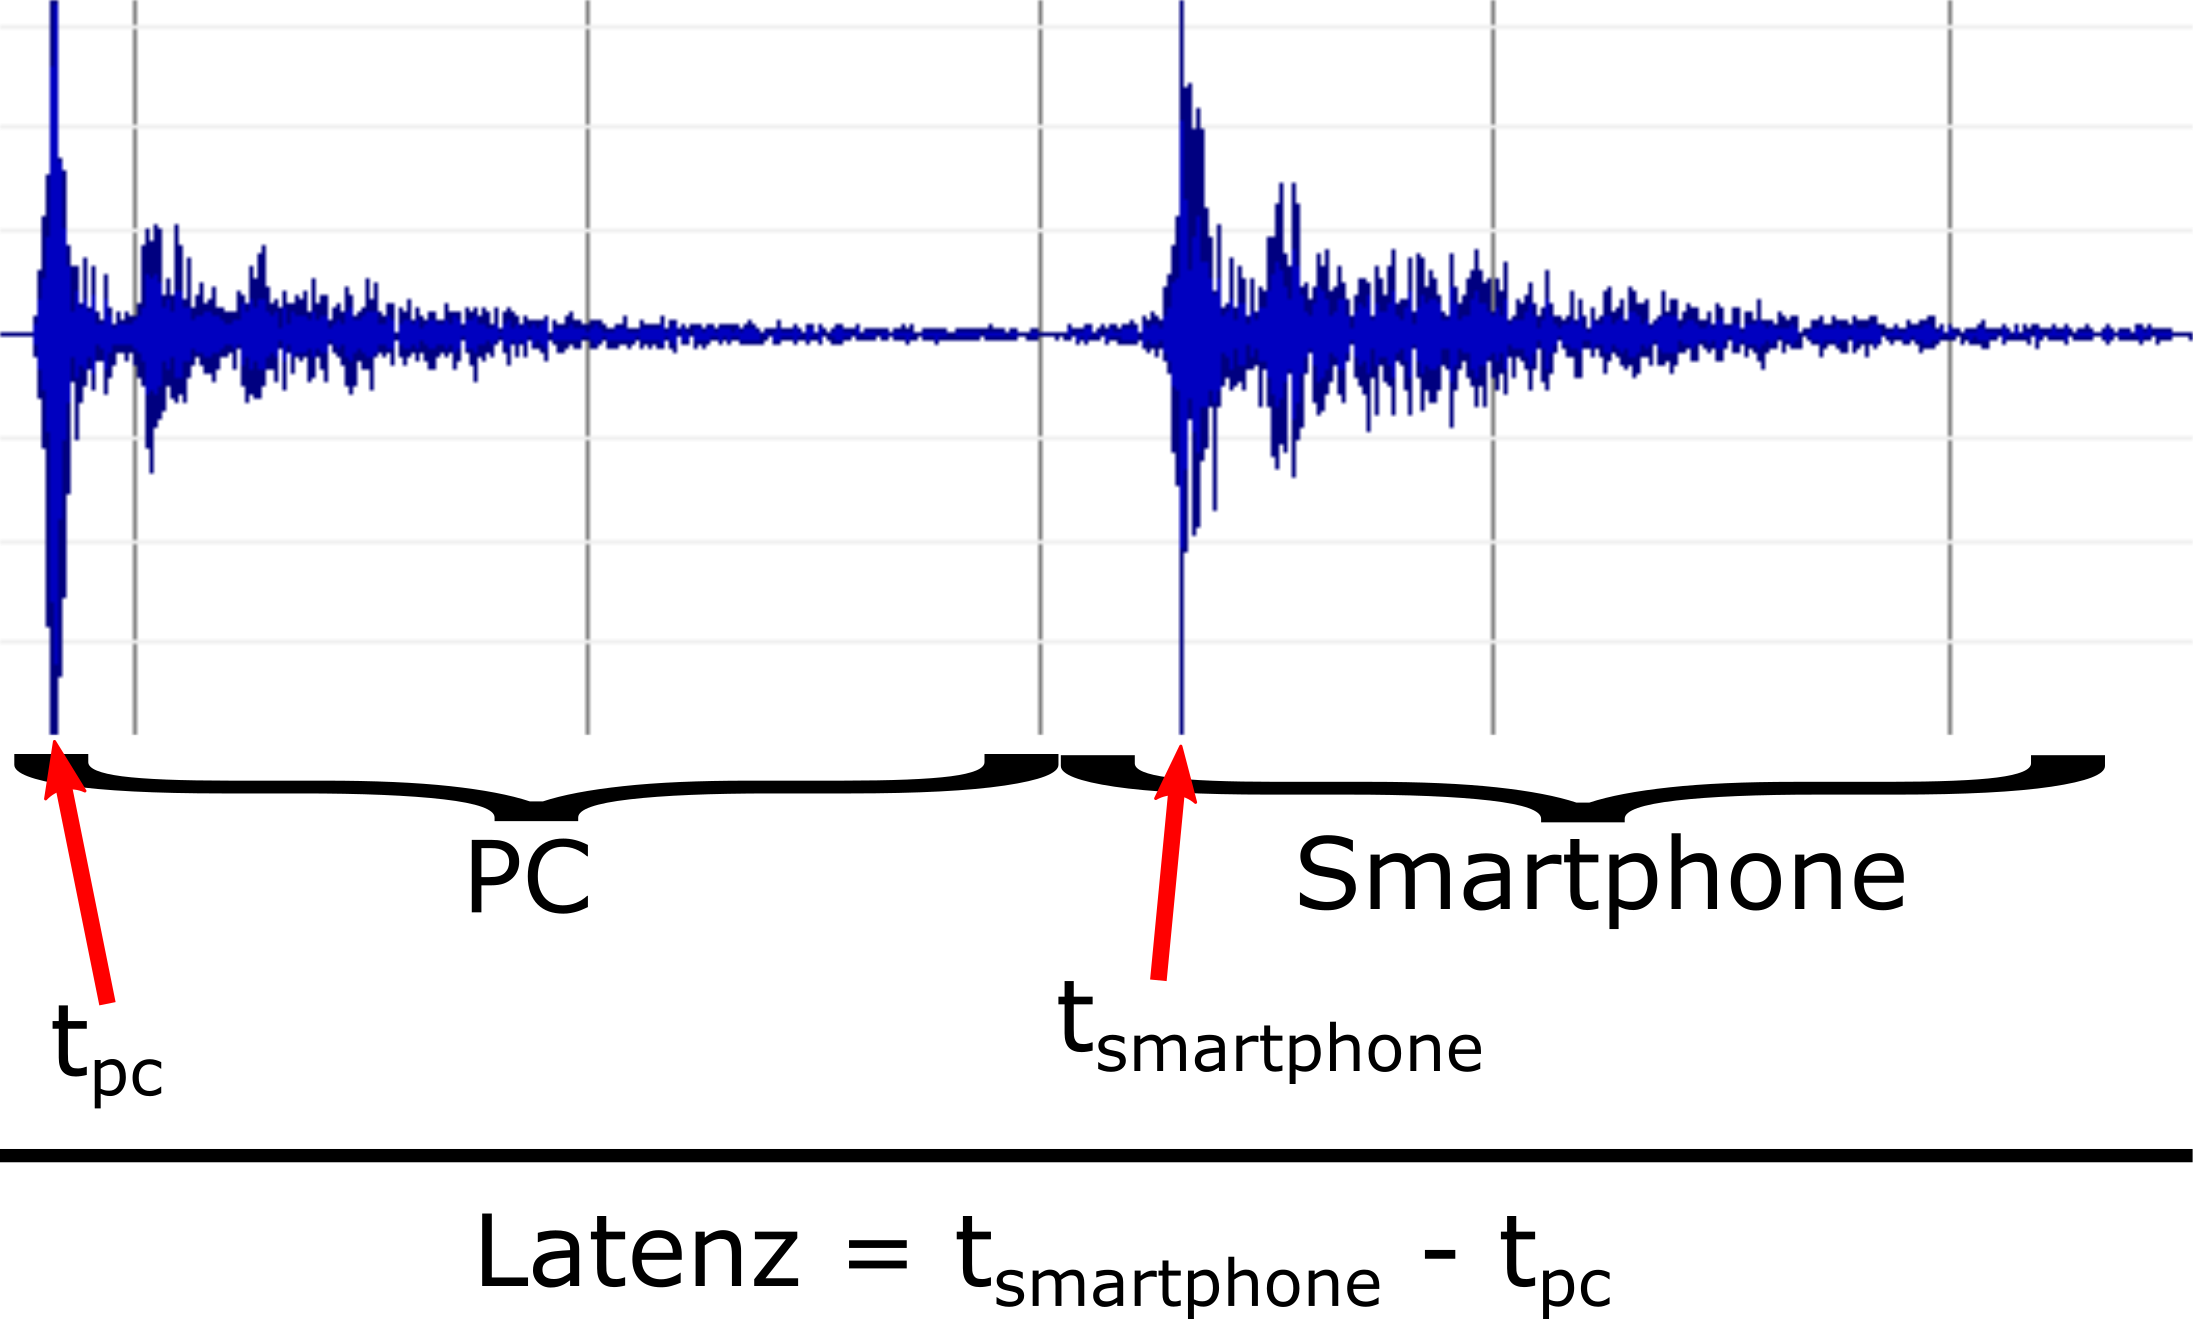
\includegraphics[width=0.7\textwidth]{img/spektrogramm.png}
		\caption{Bestimmung der Latenz anhand des Spektrogramms der Mikrofonaufnahme}
		\label{fig:spektrogramm}
	\end{center}
\end{figure}

Es wurden 30 Latenzmessungen pro Anwendung pro Smartphone aus den Leistungsklassen LOW (Samsung Galaxy S3 neo), MID (Samsung Galaxy S5) und HIGH (OnePlus 2) durchgeführt. Verwendet wurde ein PC mit Intel i7-3770k Prozessor. Die Qualität der Drahtlosübertragung kann die gemessene Latenz erheblich beeinflussen. Um den Einfluss der Übertragungsqualität einzuschränken, wurde für alle Messungen auf eine WiFi-Direct-Verbindung zurückgegriffen. Mithilfe der Anwendung Wifi Analyzer wurde zudem die Chance verringert, dass es während des Testens zu durch Interferenz verursachte Probleme kommt. Es wurde darauf geachtet, dass Audioqualität (48 kHz Stereo) und Puffergrößen bei allen Anwendungen gleich konfiguriert sind.

\section{Resultate}
Die in Abbildung \ref{boxplots} dargestellten Boxplots zeigen die Ergebnisse der insgesamt 9 Testreihen aufgeteilt auf die drei Leistungsklassen (LOW, MID, HIGH).


\begin{figure}[H]
\begin{subfigure}[b]{0.5\textwidth}
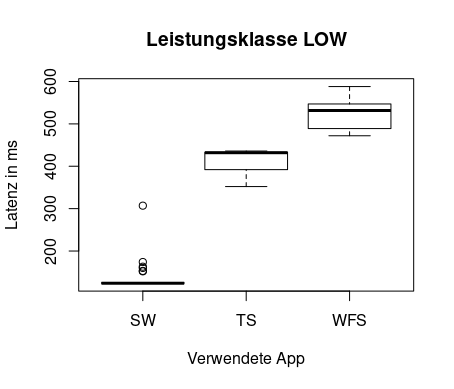
\includegraphics[width=\textwidth]{img/boxplotlow.png}
\end{subfigure}
\begin{subfigure}[b]{0.5\textwidth}
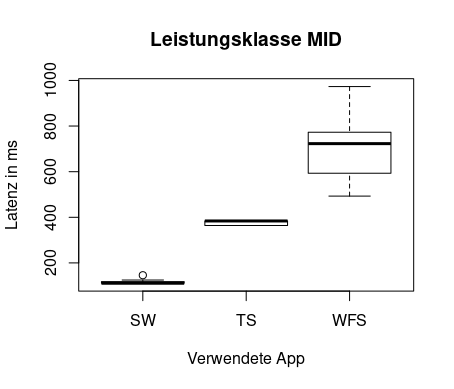
\includegraphics[width=\textwidth]{img/boxplotmid.png}
\end{subfigure}
\begin{subfigure}[b]{0.5\textwidth}
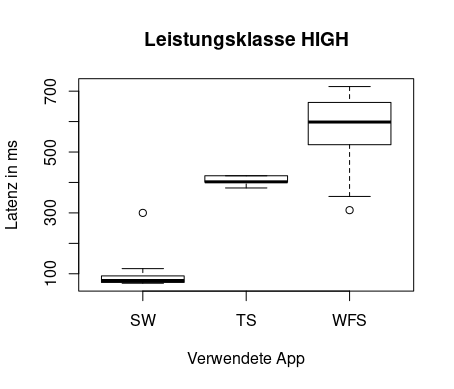
\includegraphics[width=\textwidth]{img/boxplothigh.png}
\end{subfigure}
\caption{Testergebnisse der insgesamt neun Testreihen}
\label{boxplots}
\end{figure}

Nach bloßem Betrachten der Ergebnisse lässt sich die Tendenz verzeichnen, dass bei allen Leistungsklassen SW die geringste Latenz aufweist. Die anschließende statistische Auswertung soll also folgende Hypothesen bestätigen:

\begin{itemize}
\item SW weißt eine geringere Latenz auf als TS.
\item SW weißt eine geringere Latenz auf als WFS.
\end{itemize}

Die Ergebnisse der einzelnen Testreihen wurden dem Shapiro-Wilk Test unterzogen, um auf Normalverteilung zu überprüfen. Nur die Datenreihe der Leistungsklasse LOW und der App WFS verzeichnete dabei einen p-Wert über dem Signifikanzniveau von 0.05 mit einem Wert von 0.06187, wodurch es sich wahrscheinlich um eine Normalverteilung handelt. Bei allen anderen Datenreihen ist anzunehmen, dass diese nicht auf einer Normalverteilung basieren.

In den meisten Datensätzen konnten wir keine Normalverteilung statistisch signifikant feststellen, allerdings sind in jeder Datenreihe 30 Ergebnisse enthalten. Dadurch ist es möglich, pro Geräteklasse einen T-Test zur Überprüfung der Hypothesen durchzuführen. Dabei ist zu beachten, dass der Datensatz von SW jeweils zweimal verwendet wird. Um das Problem des multiplen Testens zu umgehen, wird die Bonferoni-Korrektur angewandt. Dadurch wird das Signifikanzniveau halbiert und somit auf 0.025 gesetzt. Es werden pro Leistungsklasse zwei einseitige T-Tests durchgeführt, welche die Latenzen von SW mit TS und von SW mit WFS vergleichen.

\begin{table}[h]

\begin{tabular}{l|p{2cm}|p{2cm}|p{2cm}}
& LOW & MID & HIGH \\
\hline
SW/TS & t = -35.542; \newline df = 52.287; \newline p-value $< 2.2e-16$ & t = -116.18 \newline df = 51.875; \newline p-value $< 2.2e-16$ & t = -40.896 \newline df = 35.239; \newline p-value $< 2.2e-16$\\
\hline
SW/WFS & t = -44.652; \newline df = 57.64; \newline p-value $< 2.2e-16$ & t = -24.684; \newline df = 29.182; \newline p-value $< 2.2e-16$ & t = -24.806; \newline df = 38.176; \newline p-value $< 2.2e-16$ \\

\end{tabular}
\caption{Ergebnisse der T-Tests}
\end{table}

In allen T-Tests wird das Signifikanzniveau von 0.025 vom p-Wert klar unterschritten. Daraus folgt, dass die vorher aufgestellten Hypothesen akzeptiert werden können. Folgende 95\% Konfidenzintervalle wurden durch die T-Tests berechnet:

\begin{table}[h]

\begin{tabular}{l|p{2cm}|p{2cm}|p{2cm}}
& LOW & MID & HIGH \\
\hline
SW/TS & -Inf -0.2663635 & -Inf -0.2571063 & -Inf -0.3052234 \\
\hline
SW/WFS & -Inf -0.3753667 & -Inf -0.5284751 & -Inf -0.4623933 \\

\end{tabular}
\caption{95\% - Konfidenzintervalle der T-Tests}
\end{table}

Es kann abgelesen werden, dass in 95\% der Fälle die Latenz von SW je nach Leistungsklasse und zu vergleichender App zwischen rund 257ms und 528ms geringer ausfällt.

\section{Gefahren für die Validität}
Die größte Gefahr für die interne Validität stellt die Qualität der Drahtlosübertragung dar. Eine schlechte Verbindungsqualität kann eine höhere Latenz verursachen. Mithilfe der Anwendung WiFi Analyzer wurde über den gesamten Testzeitraum sichergestellt, dass keine anderen WiFi-Sender wesentlich aktiv sind. Jedoch konnte damit nicht sichergestellt werden, dass Sender, die eine andere Drahtlosübertragungstechnik wie 4g oder Bluetooth verwenden, zu einer Verschlechterung der Verbindungsqualität beitragen. Weiter ist die interne Validität des Experiments dadurch gefährdet, dass die Zeitwerte vom Spektrogramm von unterschiedlichen Personen anders abgelesen werden könnten. Um die Objektivität des Messvorgangs zu erhöhen, wurden alle Latenzwerte von drei Personen unabhängig abgelesen. Die maximale Abweichung zwischen den Messergebnissen unterschiedlicher Personen betrug lediglich eine Millisekunden. Durch die Wiederholung der Tests mit Smartphones unterschiedlicher Leistungsklassen wurde versucht, das Ergebnis auf eine größere Bandbreite von Smartphones verallgemeinerbar zu machen. Um die externe Validität zu erhöhen, ist es jedoch sinnvoll mit einer größeren Anzahl verschiedener Smartphones zu testen.

\section{Fazit}
Als klarer Sieger des Tests geht die App SoundWire hervor, da diese die geringste Latenz in allen Leistungsklassen aufweisen konnte. Wie auch schon in Kapitel \ref{threats} aufgezeigt, spielt die Qualität der WiFi-Verbindung eine entscheidende Rolle auf die Verzögerungszeit bei der drahtlosen Tonübertragung. In einem realen Umfeld, bei dem die Apps als Ersatz für Kabellose Kopfhörer zum Einsatz kommen sollen, muss klar nach Andwendungszweck unterschieden werden. Wird die Beschriebene Vorgehensweise beispielsweise zur Übertragung von Musik genutzt, stellt die Latenz keine Probleme dar. Die besten Latenzwerte die in unseren Tests gemessen wurden bewegten sich im Bereich knapp unter 100ms. Für Anwendungen im Filmbereich ist diese Latenz noch etwas zu groß. Eine Verzögerung von Ton- zur Videospur in dieser Größenordnung kann immer noch als störend empfunden werden. Es bleibt abzuwarten, ob in Zukunft Apps entwickelt werden, die diese Übertragungstechnik mit einer geringeren Latenz bewerkstelligen können. Außerdem ist es möglich, dass durch bessere WLAN-Technik eine Übertragung mit geringeren Verzögerungszeiten durchgeführt werden kann.

%
% ---- Bibliography ----
%
\begin{thebibliography}{}
%
\bibitem[1980]{2clar:eke}
Clarke, F., Ekeland, I.:
Nonlinear oscillations and
boundary-value problems for Hamiltonian systems.
Arch. Rat. Mech. Anal. 78, 315--333 (1982)

\bibitem[1981]{2clar:eke:2}
Clarke, F., Ekeland, I.:
Solutions p\'{e}riodiques, du
p\'{e}riode donn\'{e}e, des \'{e}quations hamiltoniennes.
Note CRAS Paris 287, 1013--1015 (1978)

\bibitem[1982]{2mich:tar}
Michalek, R., Tarantello, G.:
Subharmonic solutions with prescribed minimal
period for nonautonomous Hamiltonian systems.
J. Diff. Eq. 72, 28--55 (1988)

\bibitem[1983]{2tar}
Tarantello, G.:
Subharmonic solutions for Hamiltonian
systems via a $\bbbz_{p}$ pseudoindex theory.
Annali di Matematica Pura (to appear)

\bibitem[1985]{2rab}
Rabinowitz, P.:
On subharmonic solutions of a Hamiltonian system.
Comm. Pure Appl. Math. 33, 609--633 (1980)

\end{thebibliography}
\end{document}
